\section{Methods not Pursued}\label{sec:design_unused_methods}% TODO: Better name?

\subsection{Road trip}

Before the \caida and \ripe Atlas data was uncovered, an idea for gathering everywhere-to-everywhere data was conceived and seriously considered: take an enormous road trip across the United States, taking measurements along the way. The idea is simple enough in theory and in practice. Just assemble a list of websites to run traceroutes to and run constant traceroutes against them on the journey, mapping them to GPS coordinates along the way.

By the end of the trip there would be traceroutes from every point along the route to all the different sites in the list, many times over. This, it was hoped, would yield a significant amount of quality data. With two people in one car taking shifts in driving (or alternately, staying in hotels for 7-8 hours at a time), it was estimated that the entire US could be roughly circumnavigated in about 7 days.

Fortunately the \caida and \ripe Atlas data sets were discovered well before any serious planning was underway. The idea was almost immediately nixed, since it turns out that nobody actually wants to spend a week in a car.

\subsection{Network Time Protocol}

\ntp is a protocol designed to keep computer clocks around the world in sync with each other. Per the specification for the third version, \ntp is designed to "maintain accuracy and robustness" despite being implemented on "unreliable" networks with "dispersive delays" \cite{rfc1305}. As part of this protocol, the delay, or delta, between the client and server is calculated \cite{rfc5905}. Given the precise nature of this protocol, it would be ideal for this project, which is focused on measuring the network time between geographic locations. The only requirements would be a geographically diverse set of \ntp servers willing to provide the calculated delay values to their peers. Luckily, both parts of this requirement are met -- sort of.

The \ntp specification details a server mode, mode 6, that allows for "remote control queries" which provide a way for remote management of certain aspects of the server \cite{Haberman2019Control4}. One of the these queries, the \texttt{peers} command, prompts the server to return a list of its peers, along with calculated statistics for these peers -- including the delay. \autoref{fig:sample_ntpq} is an example of such a command using the \texttt{ntpq} tool (with some returned fields removed for formatting).

\begin{figure}[h]
    \centering
    \begin{minted}{bash}
    >ntpq -c peers 127.0.0.1
         remote           refid      delay   offset  jitter
    =======================================================
    *ntp1.wpi.edu    130.215.32.36   0.851   -0.076   0.134
    +ntp2.wpi.edu    130.215.32.36   0.646   -0.366   0.182
    +ntp3.wpi.edu    130.215.144.33  1.376    0.711   0.261
    \end{minted}
    \caption{Sample NTP Mode 6 \texttt{peers} command output}
    \label{fig:sample_ntpq}
\end{figure}

As the example shows, the \texttt{peers} command response includes both the delay and the jitter calculations for each peer. Coupled with \ip geolocation, requesting the peers from a list of mode 6 \ntp servers would be a straightforward way of getting point to point measurements. And there is no shortage of \ntp servers with mode 6 enabled in the United States: according to the ShadowServer Foundation, which conducts period scans for such servers, as of January 22nd, 2020, there are 522,415 such servers in the country \cite{TheShadowserverFoundationNTPProject}. Additionally, as \autoref{fig:ntp_mode_6_us_map} shows, they are distributed across most of the country.

\begin{figure}[H]
    \centering
    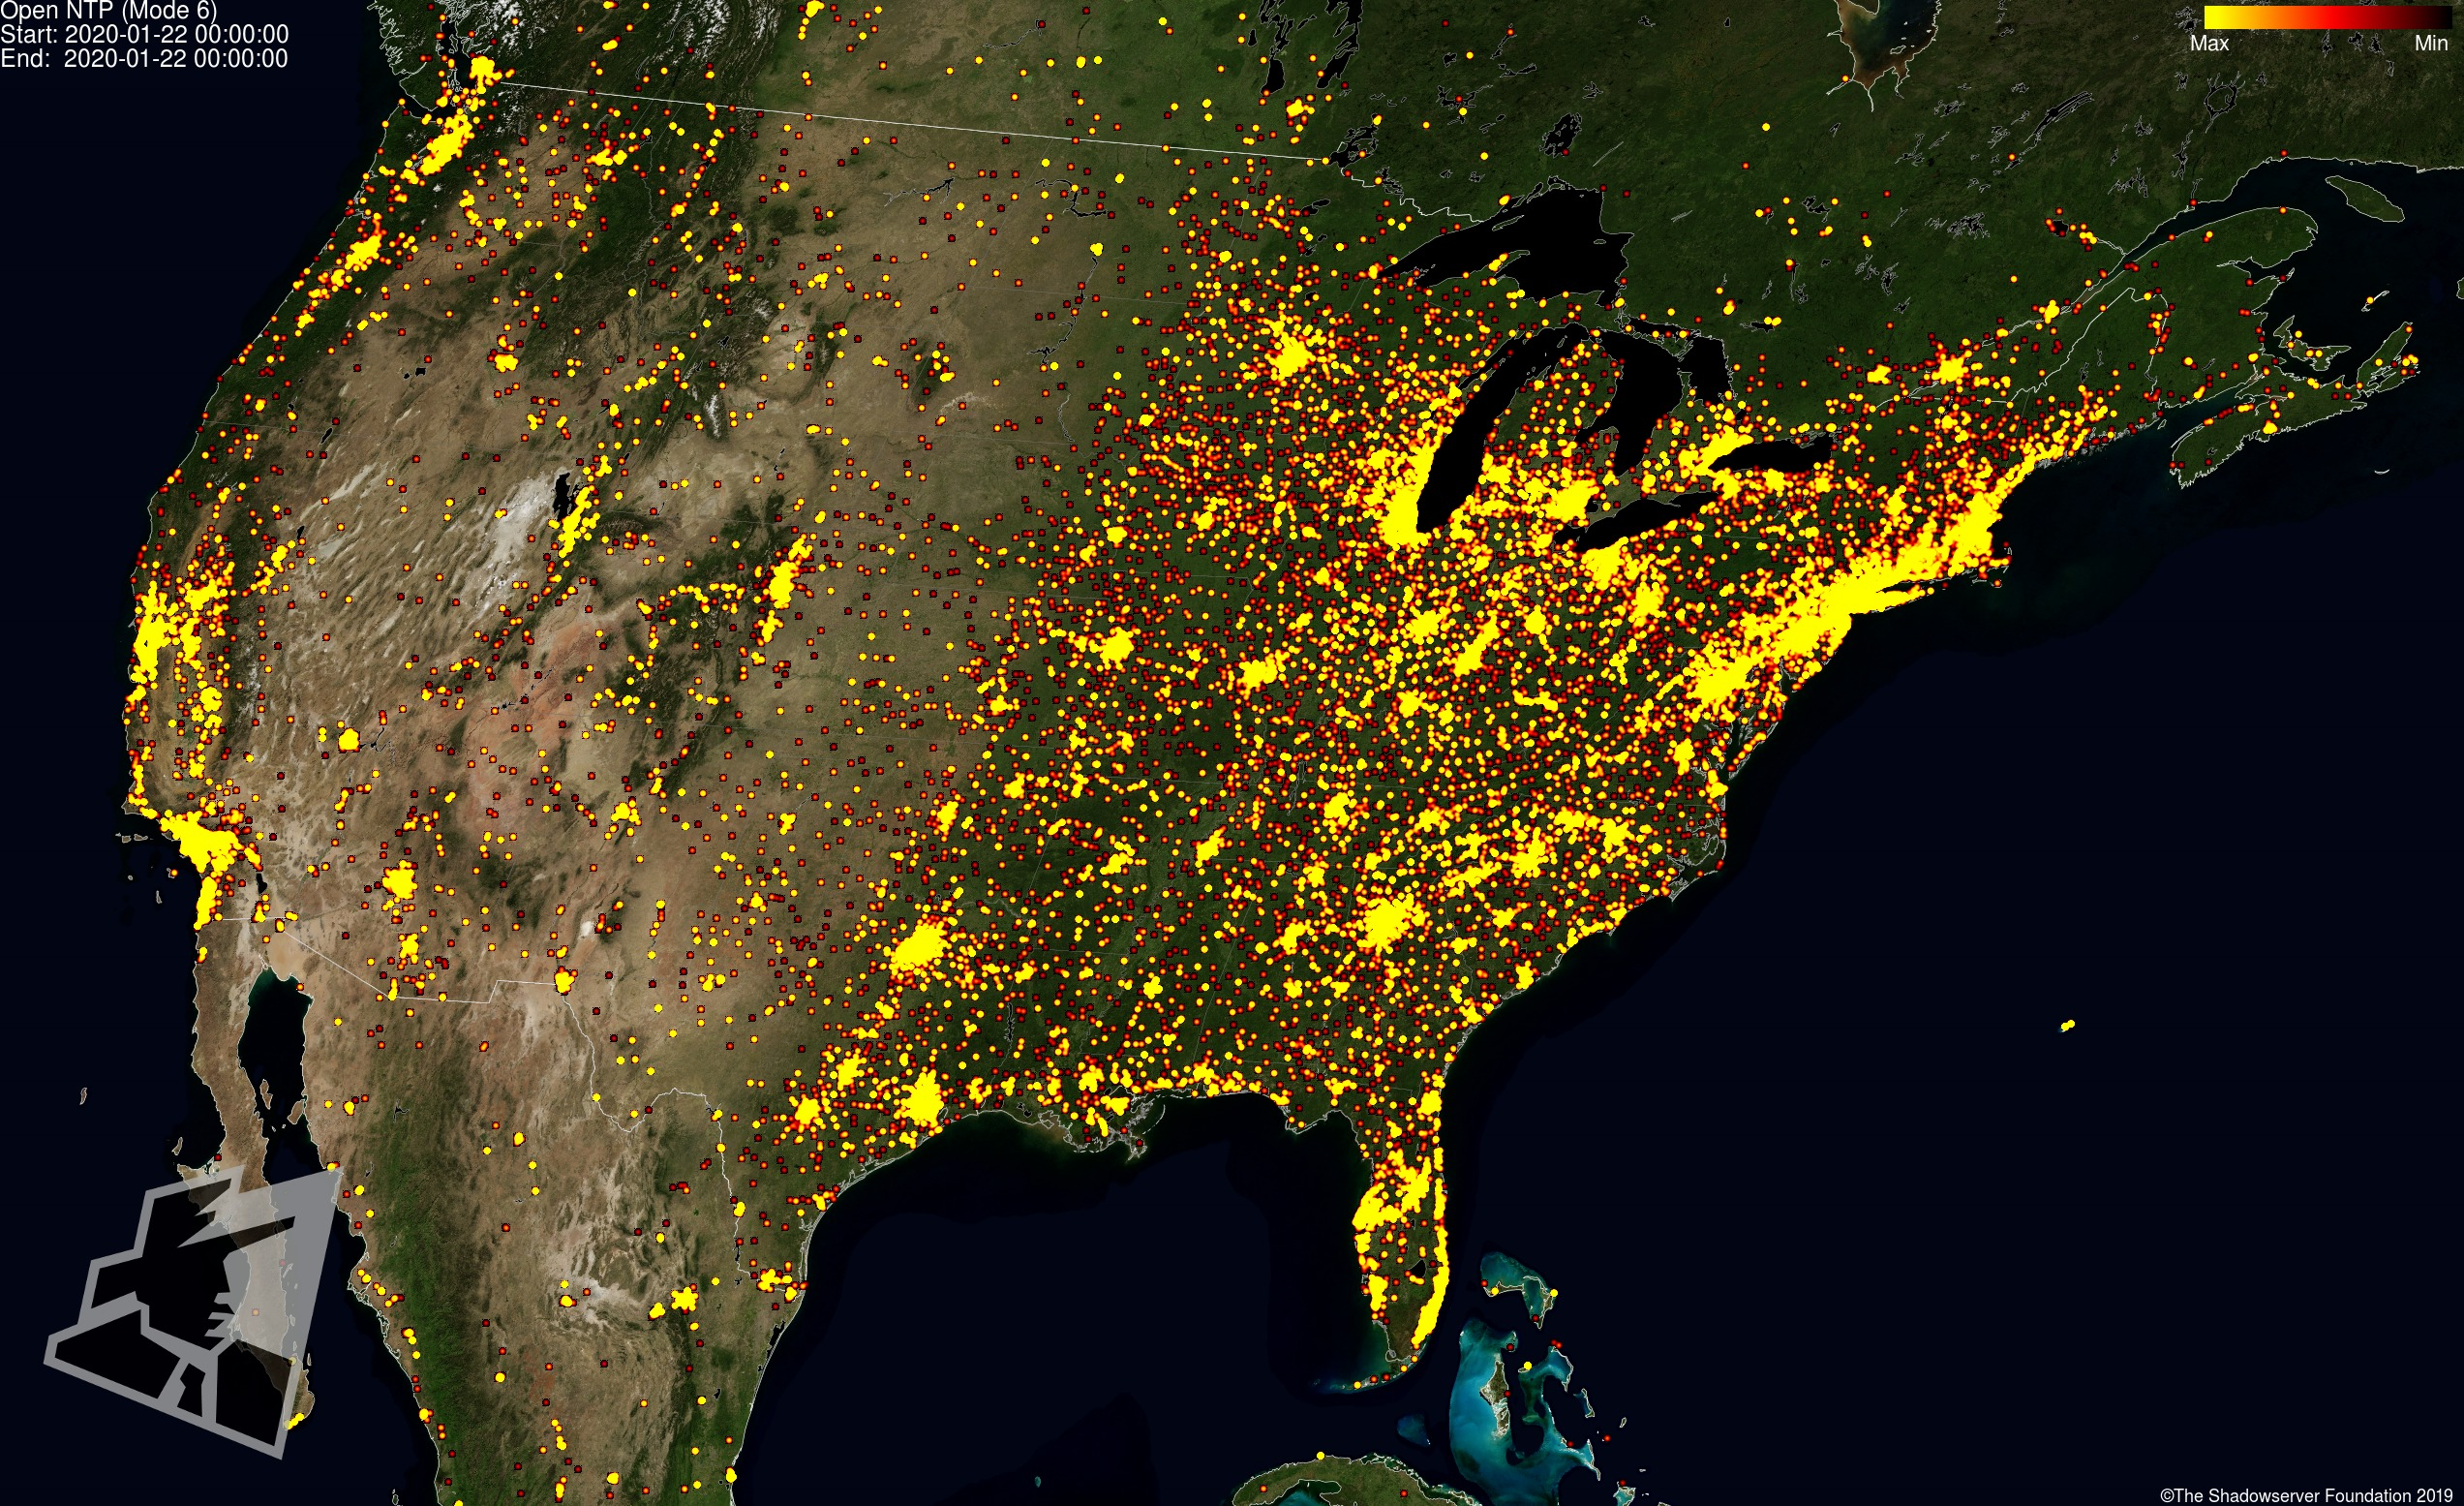
\includegraphics[width=\textwidth]{images/ntpversion_united_states_current.jpg}
    \caption{Distribution of \ntp Mode 6 Servers in the US}
    \label{fig:ntp_mode_6_us_map}
\end{figure}

In theory, using these servers and conducting a simple survey of the delay times to each of their peers would be an ideal method for this project. Unfortunately, one of the commands included in mode 6 makes the servers vulnerable to being exploited for use in amplified \ddos attacks \cite{USDepartmentofHomelandSecurity2014NTPCVE-2013-5211}. Thus, despite performing frequent scans for mode 6 servers, the ShadowServer Foundation does not publish a list of such servers, since doing so would be a security risk. We found no other source of potential servers and proceed to attempt our own scan of potential \ip ranges. While we found some potential servers, many lacked any peers and the search was time intensive. Future work may include this method, as it is promising, provided a list of potential servers is available, or more time can be dedicated to scanning for them.

\subsection{ISP Mapping}
FCC fixed broadband deployment map
 The \FCC maintains a map of broadband internet deployment across the United States \cite{FederalCommunicationsCommission}. This map is drawn at a census block level and only considers residential broadband.
